\subsection{design}\label{subsec: vm-design}
OlaVM is a virtual machine for the zero-knowledge(ZK) proof.The design principle is ZK friendly and user friendly.
To achieve the targets, designs have been made in the following aspects:

\begin{itemize}
    \item \verb|minimize instructions set|
    \item \verb|use prophet to minimize trace length|
    \item \verb|minimize general register number|
    \item \verb|memory segment|
\end{itemize}

\subsubsection{minimize instructions set}
Every instruction(include builtin instruction) needs one column in cpu trace table to present and need different constrains.So the design minimizes instructions set for minimizing the columns in cpu trace table.
OlaVM use 21 instructions, reference: \ref{table:instruction-set}. \\
One of the main features of the reduced instruction set architecture (RISC) adopted by OlaVM is that there are fewer instruction sets, compared with the complex instruction set architecture (CISC, Complex Instruction Set Computer).
For the difference between the two, please refer to \href{https://cs.stanford.edu/people/eroberts/courses/soco/projects/risc/risccisc/}{RISC vs. CISC }.
The main reason for choosing the RISC architecture is to obtain ZK-Friendly, mainly from two aspects:

\begin{itemize}
    \item \verb|RISC architecture can reduce the number of constraint polynomials|
    In ZKVM, there is a critical constraint:  CSTC(CPU State Transition Constraint).It is used to constrain OlaVM state transition before and after an instruction is executed.
    As shown in Figure \ref{fig:cstc_example}, When a VM executes an instruction, it changes the state of the associated registers Therefore, to ensure the correctness of VM execution, Olavm use circuit to constrain the register state transition.
    \begin{figure}[!htp]
        \centering
        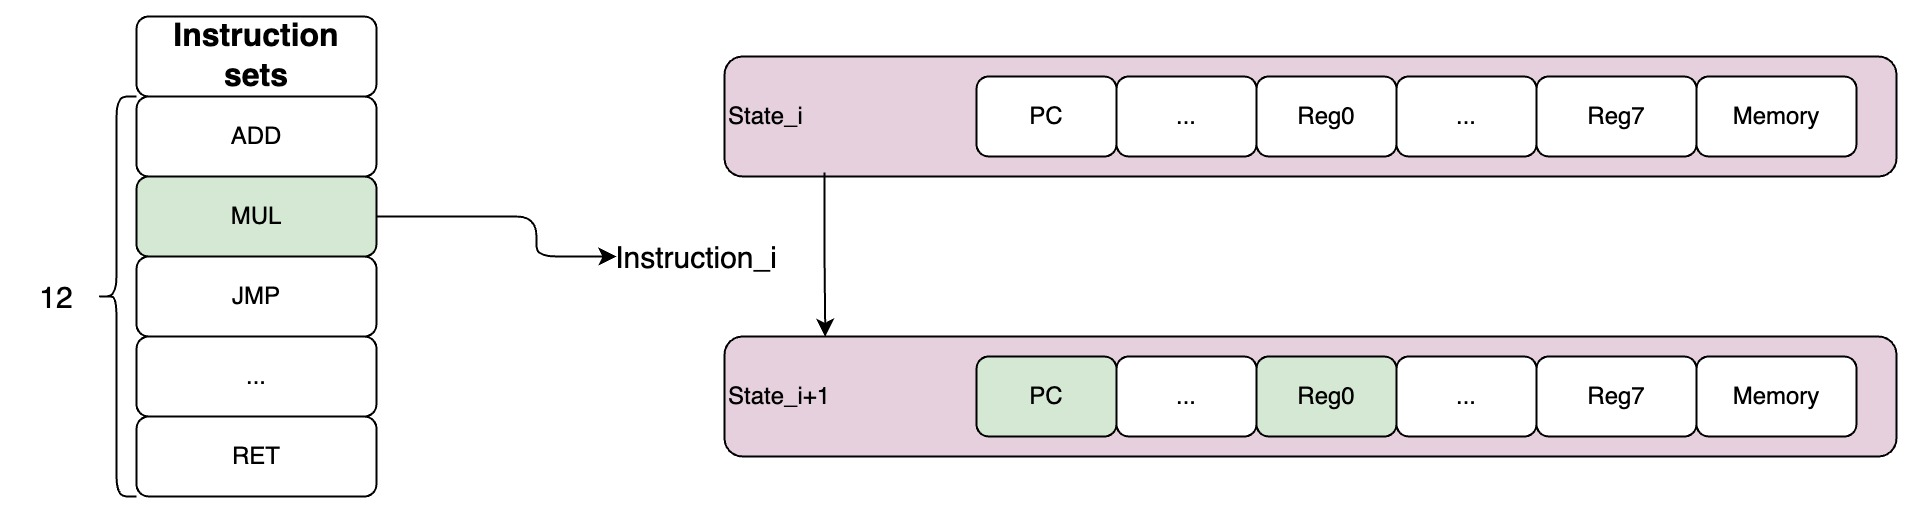
\includegraphics[width=1\textwidth]{cstc_example}
        \caption{CPU trace snippet}
        \label{fig:cstc_example}
    \end{figure}
    The cpu trace table as below \ref{table:cstc_trace_snippet}. When OlaVM execute three instructions(ADD, MOV, JMP), the register state have been changed.For example,PC register state transitions for the three instructions:
    \begin{align*}
    \textit{ADD}: \textit{pc}_{i+1}  = \textit{pc}_i + 1\\
    \textit{MOV}: \textit{pc}_{i+1} = \textit{pc}_i+ 2\\
    \textit{JMP}: \textit{pc}_{i+1}=2
    \end{align*}
    OlaVM must design as many as constraints to handle all instructions which called CSTC above.
    For this example, the constraint of updating PC register state when OlaVM executes every instruction as follows:
    \begin{align*}
        \textit{pc}_{i+1}=\textit{Sel}_{\textit{JMP}}* \textit{IMM}+(1 - \textit{Sel}_{\textit{JMP}})(\textit{pc}_i + 1 + \textit{Sel}_{\textit{IMM}})
    \end{align*}
    \begin{table}[!ht]
        \resizebox{\textwidth}{!}{
            \begin{tabular}{|c|c|c|c|c|c|c|}
                \hline
                \textit{Clock}  & \textit{PC} & \textit{Instruction} & \textit{...} & \textit{reg0} & \textit{reg1} & \textit{reg2} \\ \hline
                ... & ... &  ...  & ... & ... & ... & ... \\ \hline
                i & 8 &  ADD r0 r0 r1 & ... & 1 & 2 & 0 \\ \hline
                i+1 & 9 e &  MOV reg2 3 & ... & 3 & 2 & 0 \\ \hline
                i+2 & 11 &  JMP 2  & ... & 3 & 2 & 3 \\ \hline
                i+3 & 2 &  ...  & ... & 3 & 2 & 3 \\ \hline
            \end{tabular}}
        \caption{cpu trace table snippet}
        \label{table:cstc_trace_snippet}
    \end{table}
    \item \verb|Most operations require a small portion of the instruction set|
\end{itemize}

\subsubsection{use prophet to minimize trace length}
There are one application scene: some algorithm is difficult to computation but ease to verify.For example: compute the square root of a radicand.
To implement Newton's method  need more then 20 instructions, but by contrast, verify a result is the square root of a radicand is succinct.
ZKVM only need to use the result multiply itself to get a product, and verify if the product is equal to the radicand.Only use two instructions.
By the second algorithm, how to compute the square root is no matter to ZK circuit and user.
The process of computation is wrapped up in prophet segment and not need to be verified by ZK circuit.
ZK circuit only need to verify the succinct logic $\texttt{result} /cdt \texttt{result} == \texttt{radicand}$.
Use OlaVM to execute two algorithm and generate ZK proof, The second algorithm is 10 times faster than the first traditional algorithm.
reference: \ref{subsec: prophet-interpreter}

\subsubsection{minimize general register number}
Every register need one column in cpu trace table to present and need different constrains.So the design minimize the number of register to minimize the columns in cpu trace table.
OlaVM use 9 general registers and 2 system registers(PC, PSP),  reference: \ref{subsec: zkvm-executor-register}.

\subsubsection{memory segment}
THe memory design is influenced by the prophet.To ensure that the memory trace table can be written by prophet without use instructions,the memory space need be partitioned into several segment.
The prophet segment is write-once for constraint. reference: \ref{subsec: ola-memory}